\documentclass[compsoc]{IEEEtran}
\IEEEoverridecommandlockouts
\usepackage{cite}
\usepackage{caption}
\usepackage{amsmath,amssymb,amsfonts}
\usepackage{algorithm}
\usepackage[noend]{algpseudocode}
\usepackage{textcomp}
\usepackage{xcolor}
\usepackage{comment}
\usepackage{array}
\def\BibTeX{{\rm B\kern-.05em{\sc i\kern-.025em b}\kern-.08em
    T\kern-.1667em\lower.7ex\hbox{E}\kern-.125emX}}
\usepackage{stfloats}
\usepackage{float}
\usepackage{hhline}
\usepackage{booktabs}
\usepackage[export]{adjustbox}

\usepackage[caption=false,font=footnotesize]{subfig}
\usepackage{graphicx}
\graphicspath{ {./images/} }

\usepackage{pgfplots}
\pgfplotsset{width=7cm,compat=1.8}
\captionsetup{format=default, font=footnotesize, labelfont=bf}


%%%%%%%%%%%%%%%%
\begin{document}
%%%%%%%%%%%%%%%%
\title{Feature-Based Used Car Price Predictor Using Linear Regression and Support Vector Machines}

\author{Parker~Smith
\thanks{P. Smith is with the College of Computing and Software Engineering, Kennesaw State University, Marietta, GA, 30060 USA. Email: psmit216@students.kennesaw.edu}}

%%%%%%%%%%%%%%%
\IEEEtitleabstractindextext{%
    
    \begin{abstract}
    Cars are often the second largest purchase that most people make. Therefore, for a car purchaser, it is important to know how much a specific vehicle truly costs and whether the price they are paying is inflated. In addition, car salesmen must know an accurate price of the car they are selling so they can make the most profit from their sale. Finally, private car sellers wish to sell their car quickly, yet not under-price their vehicle. This problem of predicting the price of a car can be solved by inputting the car's features through a machine learning algorithm. In doing so, all users will be able to obtain an objective view of how much the vehicle is worth. Current models allow users to input a Vehicle Identification Number or enter a make and model of a vehicle to get a price result. However, these models tend to have accuracies lower than 85\%. This project attempts to solve this problem in a different way by implementing two models: Linear Regression and a Support Vector Machine. The primary evaluation metrics for these models are their $R^2$ accuracy, their Mean Square Error, their Root Mean Square Error, and their training time. Both models have a large dataset of vehicle features such as make, model, condition, transmission type, color, odometer reading, and many others. With this larger feature set, both models achieved better results when compared to the baseline project by Kumbar, Gadre, and Nayak. The baseline's best model had an $R^2$ accuracy of 87\% and a training time of 15 minutes while this project's models had an $R^2$ accuracy of 97\%, a Root Mean Squared Error of \$1,450, and a training time of less than a minute. Due to the larger feature set and improved models, this project's Linear Regression and Support Vector Machine models are both accurate enough to predict the approximate value of a car using only an input of features.
    \end{abstract}
    %%%%%%%%%%%%%%%%
    \begin{IEEEkeywords}
    Computer science, data analysis, data processing, deep learning, land vehicles, linear approximation, machine learning, neural networks, optimization, performance analysis, python, supervised learning, transportation, vehicles
    \end{IEEEkeywords}
    %%%%%%%%%%%%%%%%%%%%%%%
}

\maketitle
\IEEEdisplaynontitleabstractindextext
\section{Introduction}
As the second largest purchase most people make, cars, and the car industry, are very important to the economy. In 2018, motor vehicles and parts accounted for \$521.5 billion of the US's Gross Domestic Product (GDP) \cite{website:auto_industry}. Of course, due to the high economic impact and comparatively large price tag of most cars, many people are hesitant when it comes to purchasing a new car. The average price of a new car is \$46,426, whereas the average price of a used car is only \$30,000 \cite{website:car_prices}. This price gap has led many consumers to lean towards purchasing used cars. However, determining an optimal price for a used car is a difficult task. There are many factors to weigh including economic factors, make, body style, mileage, transmission type, condition, and more \cite{website:value_factors}. A consumer must weigh all these factors, along with the listed price of the car, to determine whether they wish to purchase that car or not. This project intends to create a Linear Regression model \cite{model:multiple_linear_regression} to allow any user to quickly determine an accurate price for a used car based solely on its features.

This is important for consumers because it allows them to save time when purchasing a new car. Currently, a consumer must find the right kind of car for them, then search through hundreds of listings to find a price that they feel is appropriate. Unfortunately, this price may still be excessive. Using machine learning, a consumer could simply input the features they are looking for and the algorithm would output a fair and reasonable price for that type of car. 

Devising a fair used car price is also important for car salesman. Their primary goal is to gain as much profit as possible off of the sale of a used car while still maintaining a price that attracts buyers. If they price too high or too low, they either cannot find buyers or they make too little profit off of a vehicle. Similar to consumers, an algorithm that will display an appropriate listing price based on the features of the cars they have in stock would be optimal for professional salesmen.

Another party that can benefit from this project is private car sellers. Currently, private sellers have difficulty in the car market as they often have an over-inflated sense of how much their car is worth \cite{website:private_seller}. Using the models from this project, private sellers could determine an accurate price for their vehicle based on some of its features including condition and mileage, and become competitive on the market. This would attract more buyers and lead to much quicker sales.

Currently, users can use websites such as Kelly Blue Book \cite{website:kbb}, TrueCar \cite{website:truecar}, and CARFAX \cite{website:carfax} to input a car's Vehicle Identification Number (VIN) and licence plate number and have an approximate price given based on features extrapolated from the VIN number. This is an effective method if a consumer or private seller is attempting to look up a value for a specific car, but not helpful if the user is just trying to figure out what is a good deal and what is not. This is also a suitable solution for car salesmen who always have the VIN and licence plate numbers of their cars in stock.

The baseline for this project builds upon current car price websites by specifically using features from a car, rather than just a VIN, to predict the car's price. This allows for a more general estimate. The baseline project is from a report published by Kumbar, Gadre, and Nayak \cite{baseline}. The dataset for their model contains 1.2 million vehicle entries with the Mileage, VIN, Make, Model, Year, State, and City features for each vehicle \cite{original_dataset}. In the report, Kumbar, Gadre, and Nayak compare seven different methodologies to find which one provided the most accurate vehicle price: Linear Regression \cite{model:multiple_linear_regression}, Random Forest \cite{model:random_forest}, Gradient Boost \cite{model:gradient_boost}, XGBoost \cite{model:xg_boost}, LightGBM \cite{model:light_gbm}, KMeans + Linear Regression \cite{model:kmeans_linear_regression}, and a Deep Neural Network \cite{model:neural_network}. The results from the baseline project showed that Linear Regression was the preferred model with the highest $R^2$ score for the lowest training time, with KMeans + Linear Regression as the second best.

The baseline project was lacking, however, in several areas. First, and most important, the training times for all of the baseline's models are too long. For Linear Regression \cite{model:kmeans_linear_regression}, one of the fastest and simplest models, the training time is 15 minutes. That is much too long for a user to wait to get a result. Another fault with the baseline project is the lack of high accuracy. The best $R^2$ score for the testing data is 88\%. That leaves 12\% error, which could cost a user hundreds or even thousands of dollars. Finally, the baseline project's dataset is lacking in features. While the dataset is large, containing over 1.2 million entries, it contains only 5 usable features \cite{original_dataset}. This is not nearly enough to determine an accurate result from such a diverse list of cars.

This project's intended purpose is to solve consumers, private car sellers, and car salesmen's problems with used cars by building upon the foundation of the baseline project. This project intends to improve upon the lack of features in the baseline project's dataset by finding a dataset with more features such as vehicle condition and transmission type. This will allow for a better estimation, even if there are fewer datapoints. Overall, this project will eliminate the manual activity of searching through used car listings to find an optimal price: a process which tends to be quite inaccurate both for all users. Hopefully, a clear relationship will develop between a car's features and it's price that can be developed into an easy-to-use model.


%%%%%%%%%%%%%%%%%%%%%%%
\section{Related works} 
Many other studies have been done in regards to predicting the price of used cars through machine learning. In a conference paper by Pal, Arora, Kohli, Sundararaman, and Palakurthy \cite{article:relatedwork1}, they attempt to solve this problem using a Random Forest \cite{model:random_forest} model. They found that, through using a supervised Random Forest method with 500 Decision Trees that chose highly correlated features, they could achieve a training accuracy of 95.82\% and a testing accuracy of 83.63\%.

In a different article \cite{article:relatedwork2}, Pudaruth used four different models to predict a used car's price based off of its features: Multiple Linear Regression \cite{model:multiple_linear_regression}, K-Nearest Neighbors (KNN) \cite{model:k_nearest_neighbors}, Decision Trees \cite{model:decision_trees}, and Naïve Bayes \cite{model:naive_bayes}. Pudaruth's work is unique in that he uses a mix of regression and classification models to attempt to solve a problem that cannot naturally be divided into classes. Ultimately, though he attempted to overcome this obstacle by creating price ranges, his results are inconclusive. The Mean Absolute Error (MAE) for each of his models varies per car model from 27,000 to 45,000, and his classification models had an accuracy between 60 and 70\%.

Another model, this time by Wijnhoven and Plant \cite{article:relatedwork3}, used Sentiment Analysis \cite{model:sentiment_analysis} to determine car sales rather than using a car's features. This model compared social media posts and Google Trends data with a linear regression model of eleven car types on the Dutch market. The results showed that Google Trends data, along with general attention about a car model, showed a significant impact on sales while social media did little.

This model by Mazumdar \cite{article:relatedwork4} is based upon Multiple Linear Regression \cite{model:multiple_linear_regression} and consists of a dataset of 370,000 cars scraped from eBay. The feature set includes body style, mileage, a damage value, make and model, gear type, and much more. Ultimately, the resulting linear model used a subset of the total feature set to more accurately portray all types of vehicles. The result from the model was an $R^2$ score of .81, which Mazumdar determined to be accurate for the project's needs.

Gon{\c{c}}alves created a model to predict the price of cars using the textual description of the cars \cite{article:relatedwork5}. Specifically using the unstructured, textual description in the car's listing, he achieved an $R^2$ accuracy score of 77\% and a Mean Squared Error (MSE) of 0.19 using a Support Vector Machine (SVM) \cite{model:svm} Model.

In a paper by Varshitha, Jahnavi, and Lakshmi \cite{article:relatedwork6}, the used car industry in India, still in it's infancy compared to other countries, is explored. The paper attempts to create a model in which no bias towards the consumer or merchandiser exists when estimating the price. Ultimately, they found the Random Forest model \cite{model:random_forest} was the most accurate with a MAE of 1.097 and and $R^2$ error value of 77\%.

In another work, Lin, Marlow, and Dixon \cite{article:relatedwork7} used a Neural Network \cite{model:neural_network}, Random Forest \cite{model:random_forest}, and Linear Regression \cite{model:multiple_linear_regression} to determine the true price of used cars on an auction website. Their results, using Root Mean Squared Error (RMSE) and $R^2$ error, led to the conclusion that both the Neural Network and Random Forest models had a satisfactory prediction, with an $R^2$ error over .5 and a low RMSE for each.

Wang, Zhang, and Wang \cite{article:relatedwork8} used a Random Forest \cite{model:random_forest} approach to predict the prices of used cars in China. Their results showed that the Random Forest model ran well, with an $R^2$ error of .98.

In attempting to predict the price of used cars, Samruddhi and Kumar \cite{article:relatedwork9} used the KNN \cite{model:k_nearest_neighbors} model. Using this model they were able to heavily optimize by constantly manipulating the K value. Through their resulting experimentation, their model achieved an $R^2$ error of 85\%


%%%%%%%%%%%%%%%%%%%%%%%%
\section{Approach (and technical correctness)}
\subsection{Selecting a Dataset}
This project began by selecting an appropriate dataset: specifically one with a large number of descriptive features with a fair amount of entries. Combined, both factors would reduce overfitting. The first option was the dataset from the baseline report \cite{original_dataset}. However, while it had a large number of datapoints, it was heavily lacking in features. This is inclined to overfitting. Upon this realization a second dataset was chosen that still contained around 500,000 datapoints while providing many more descriptive features like condition, transmission type, and general vehicle type \cite{dataset}.
\subsection{Data Preprocessing}
In preprocessing the data, several features were removed which were unique to each vehicle and did not provide information towards the price: the VIN number, the seller, and the date of sale. Another feature which had to be dropped was the trim feature because it was highly dependant on the model of the car, which would lead to an incorrect regression algorithm. The remaining features were year, make, model, body style, transmission, state the car is located in, condition of the car, the odometer reading, the exterior color, the interior color, the Manheim Market Report or wholesale value \cite{website:mmr} (MMR), and the selling price. After unifying the text data to a single format, all entries which contained an empty year, make, body style, condition, odometer reading, MMR, or selling price were dropped. This cleared up all entries which shouldn't exist. Once the outliers outside three standard deviations from the mean were removed, the data was nicely processed and nearly ready for both models as Figure \ref{fig:preprocessing} shows.

\begin{figure}[h]
    \centering
    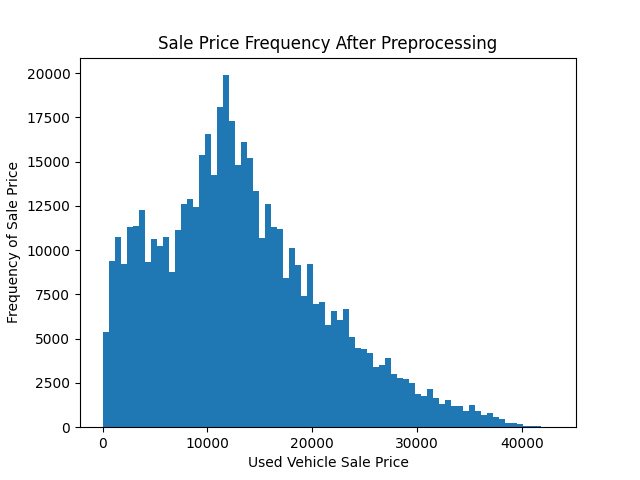
\includegraphics[width=.48\textwidth]{images/preprocessing.png}
    \caption{Distribution of data entries after preprocessing has completed}
    \label{fig:preprocessing}
\end{figure}
    
Just before use in a model, however, all text-based categorized factors such as make, model, transmission, and color are encoded to a numerical format using a One-Hot Encoding scheme \cite{model:one_hot_encoding}. This scheme allows each category in each factor to have a binary representation: turning text data into numerical data. Once this encoding is complete, the data is fully preprocessed and is ready to be used in both models.
\subsection{Plotting}
Before any models were chosen, the linearity of the data had to be determined. This would allow for an easier decision between which model would be best suited for the chosen dataset. This could most easily be achieved by plotting each feature to the price and observing whether the resulting shape was linear or not. As shown in Figure \ref{fig:mmr_linear}, there is a strong positive linear correlation between the MMR and the selling price and Figure \ref{fig:odometer_linear} shows a strong negative correlation between the reading on the vehicle's odometer and selling price. 

\begin{figure}[h]
    \centering
    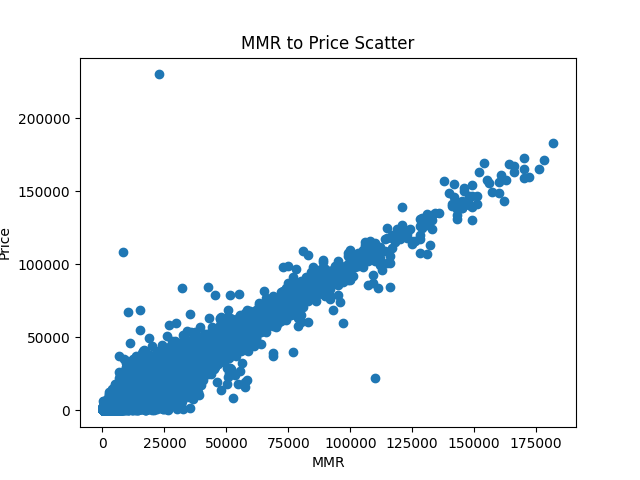
\includegraphics[width=.48\textwidth]{images/mmr_to_price.png}
    \caption{Linearity scatterplot showing the correlation between the MMR and the actual price of the car}
    \label{fig:mmr_linear}
\end{figure}
\begin{figure}[h]
    \centering
    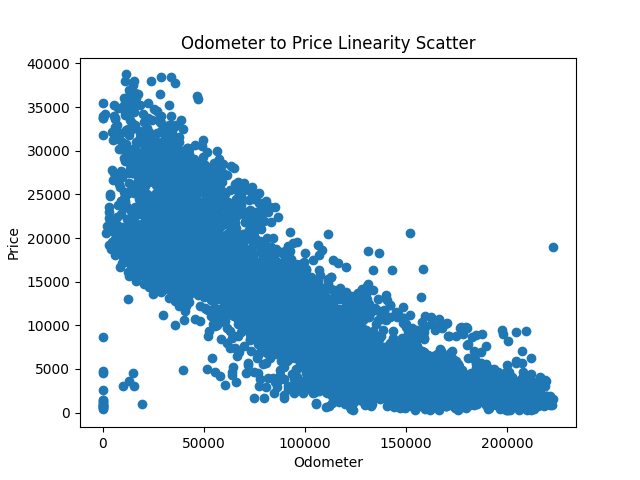
\includegraphics[width=.48\textwidth]{images/odometer_to_price.png}
    \caption{Linearity scatterplot showing the correlation between the vehicle's odometer reading and the price of the car}
    \label{fig:odometer_linear}
\end{figure}

The high linearity showcased between the price and other features proved that a linear model was the optimal choice for this project. These readings are further backed up by a heatmap of these features in Figure \ref{fig:heatmap}, showing a strong positive correlation between the selling price and MMR, a strong negative correlation between the selling price and the odometer reading, and lesser, but still significant, correlations between the selling price and the year and condition.

\begin{figure}[h]
    \centering
    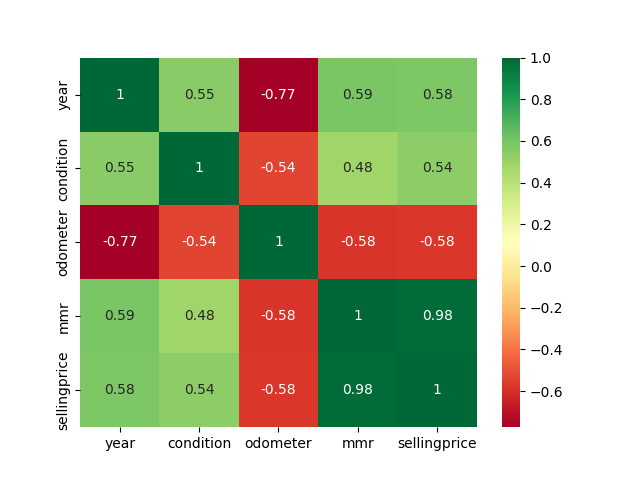
\includegraphics[width=.48\textwidth]{images/heatmap.png}
    \caption{Heatmap of the continuous features: Green = strong positive correlation, Red = strong negative correlation}
    \label{fig:heatmap}
\end{figure}

\subsection{Linear Regression Model}
Since there was such a strong linear connection between the continuous features and the price, the first model to be implemented was a linear regression model, as it is the easiest and quickest model to setup. It is a Multiple Linear Regression model \cite{model:multiple_linear_regression} with 4 continuous features, 8 categorized features, and one dependant variable. The data split was 90\% training and 10\% testing for this model since the size of the dataset was so large. The evaluation metrics for this model are the time it takes the model to train, the $R^2$ score, the MSE, and the RMSE.
\subsection{SVM Model}
In addition to the linear regression model, this project needed a secondary model as a comparison tool. An SVM \cite{model:svm} was chosen since they are fast, easy to manipulate, and work well for linear data. This model also uses the dataset of 4 continuous features, 8 categorized features, and one dependant variable. The data split was also 90\% training and 10\% testing since the dataset was the same. The evaluation metrics for this model are the time it takes the model to train, the $R^2$ score, the MSE, and the RMSE.


%%%%%%%%%%%%%%%%%
\section{Experimental results (and technical correctness)}
\subsection{Experimental Environment}
Both of the project's models were written in Python using the pandas \cite{lib:pandas}, sklearn \cite{lib:sklearn}, and matplotlib \cite{model:matplotlib} libraries. All models were run on a computer with a 4 core, 3.5GHz CPU, 16GB of memory, and an RX580 GPU with 4GB of memory. The models were not GPU enhanced. Both models ran on a data split of 90\% training and 10\% testing. The total number of samples within the dataset is 518,087. Table \ref{table:environment} encapsulates this data.

\begin{table}[h]
\centering
\caption{Summary of the environment the project was produced in}
\begin{tabular}{|l|l|l|}
\hline
CPU & 4 Core & 3.5GHz \\ \hline
Memory & 16GB & 1500MHz \\ \hline
Graphics Card & RX580 & 4GB \\ \hline
Data Split & 90\% Training & 10\% Testing\\ \hline
Sample Split & 466,278 Training & 51,809 Testing \\ \hline
\end{tabular}
\label{table:environment}
\end{table}

\subsection{Model Parameters}
For this project's Linear Regression Model, a single-epoch Multiple Linear Regression \cite{model:multiple_linear_regression} model was chosen. The model is fit once to the training data, then its accuracy is measured using the $R^2$ metric, MSE, and RMSE. The result is then reported to the user. Similarly, this project's SVM \cite{model:svm} model uses a linear kernal to emulate linear regression. The tolerance value for accepting datapoints without question is .075. After standardizing the data, the SVM model is fit once to the training data and its accuracy is measured in an identical manner to the Linear Regression model: $R^2$ accuracy, MSE, and RMSE. MSE \cite{website:mse} is measured by the equation \[\frac{\sum(y_i - \hat{y}_i)^2}{n}\] while RMSE \cite{website:rmse} is measured by the equation \[\sqrt{\frac{\sum(y_i - \hat{y}_i)^2}{n}}\]
\subsection{Results}
As Table \ref{table:results} shows, both models resulted in similar $R^2$ scores for the testing data and similar $R^2$ scores for the training data. In addition, both models have a similar MSE loss. Therefore, these models are approximately 97\% accurate when given all required features. Also, since the RMSE for each model is approximately 1,450, there is a \$1,450 dollar difference between the true price of the car and the estimated price.

\begin{table}[h]
\centering
\caption{Results after training and testing both models}
\begin{tabular}{|l|l|l|}
\hline
                     & Linear Regression & SVM \\ \hline
$R^2$ Test       & 96.84\%           & 96.74\%        \\
Accuracy           & & \\ \hline
$R^2$ Training       & 96.84\%           & 96.72\%        \\
Accuracy       & & \\ \hline
MSE Loss             & 2,022,285         & 2,097,970      \\ \hline
RMSE Loss            & 1,422.07         & 1448.44      \\ \hline
Training Time        & 44 seconds      & 38 seconds  \\ \hline
\end{tabular}
\label{table:results}
\end{table}

However, accuracy is not the only measured metric. Both models were measured in the total time it took to train the model and produce a result. Surprisingly, even with a huge dataset, both models took less than a minute to train. Both models, when compared to the baseline, are much more accurate and much quicker to train.

\begin{table}[h]
\centering
\caption{Results from the baseline project compared to this project}
\begin{tabular}{|l|l|l|l|}
\hline
Learning Algorithm & $R^2$ Test & $R^2$ Training & Training Time \\ 
    & Accuracy    & Accuracy &           \\ \hline
Linear Regression & 0.87 & 0.87 & 15 minutes \\ \hline
Gradient Boost & 0.64 & 0.64 & 130 minutes \\ \hline
Random Forest & 0.88 & 0.98 & 75 minutes \\ \hline
Light GBM & 0.81 & 0.82 & 104 seconds \\ \hline
XGBoost & 0.78 & 0.81 & 180 minutes \\ \hline
KMeans + LinReg & 0.88 & 0.89 & 70 minutes \\ \hline
Neural Network & 0.85 & 0.85 & 10 hours \\ \hline
\textbf{This Project's} & \textbf{0.97} & 0.97 & \textbf{44 seconds} \\ 
\textbf{Linear Regression} & & & \\ \hline
\textbf{This Project's SVM} & \textbf{0.97} & 0.97 & \textbf{38 seconds} \\ \hline
\end{tabular}
\label{table:baseline_results}
\end{table}

As Table \ref{table:baseline_results} shows, all of the baseline's models are significantly slower than this project's two models and none of the baseline's models' accuracies reach above 90\%. This is further shown through Figures \ref{fig:results1}, \ref{fig:results2}, and \ref{fig:results3}.

\begin{figure}[h]
    \centering
    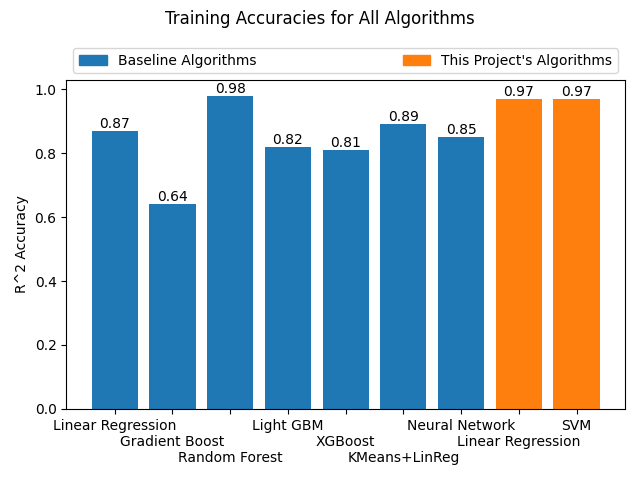
\includegraphics[width=.48\textwidth]{images/results1.png}
    \caption{$R^2$ training accuracy for both the baseline's models and this project's models}
    \label{fig:results1}
\end{figure}

\begin{figure}[h]
    \centering
    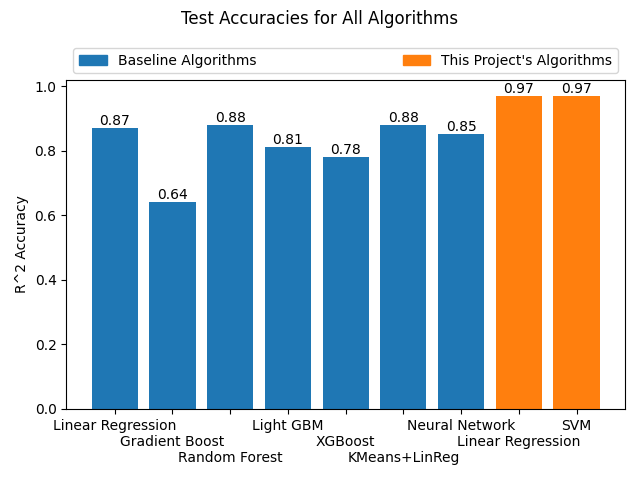
\includegraphics[width=.48\textwidth]{images/results2.png}
    \caption{$R^2$ testing accuracy for both the baseline's models and this project's models}
    \label{fig:results2}
\end{figure}

\begin{figure}[h]
    \centering
    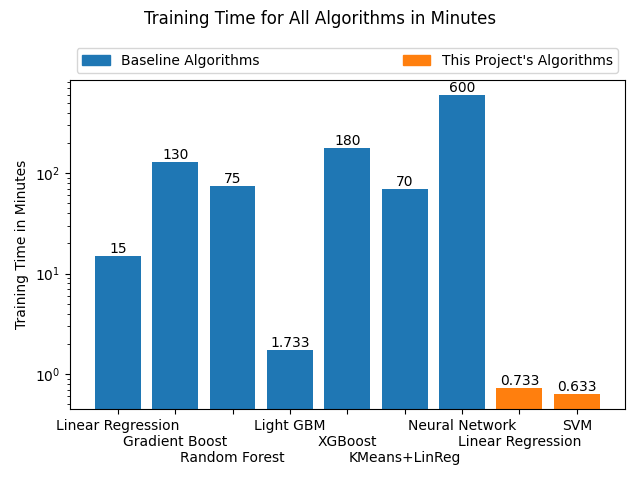
\includegraphics[width=.48\textwidth]{images/results3.png}
    \caption{Training times for both the baseline's models and this project's models}
    \label{fig:results3}
\end{figure}


%%%%%%%%%%%%%%%%%%%%
\section{Conclusion} 
As both models were highly accurate, above 95\%, both would be acceptable to predicting used car prices. The error for both models is within \$1,450. Additionally, since both models took a similar time to train, the most flexible and potentially powerful model would be the best. This project's SVM \cite{model:svm} model fits perfectly within that criteria. Since it is able to predict the prices of cars given a feature set so accurately, all users, whether individual car buyers, car salesmen, or private car sellers, can easily benefit. 

This project could be further improved upon by implementing it on a dataset with more recent car listings and a larger feature set. The more features available for training and the more recent the training vehicle listings are, the more accurate the final test results will be. Another viable addition would be to search and find accident claims based on a vehicle's VIN number. This would allow for another highly sought after feature: whether a car has even been in an accident. Finally, further optimization of the SVM \cite{model:svm}, possibly improving upon the kernel, fine-tuning the epsilon value, or implementing a better tolerance value. However, with an $R^2$ test accuracy of 97\%, the current model is certainly accurate enough for any user to predict the true value of their car.


%%%%%%%%%%%%%%%%%%%%%%%
\bibliographystyle{IEEEtran}
\bibliography{References} % (15 - 25) references

\end{document}
